\UseRawInputEncoding
\documentclass[12pt, a4paper]{article}
%\documentclass[12pt,a4paper,oneside]{book}

% --- Khai báo gói chèn code ---
\usepackage{listings}
\usepackage{xcolor}
\usepackage{multirow}

% --- Định nghĩa màu sắc cho code ---
\definecolor{codegreen}{rgb}{0,0.6,0}
\definecolor{codegray}{rgb}{0.5,0.5,0.5}
\definecolor{codepurple}{rgb}{0.58,0,0.82}
\definecolor{backcolour}{rgb}{0.95,0.95,0.92}

% --- Cấu hình style cho Python ---
\lstdefinestyle{pythonstyle}{
    backgroundcolor=\color{backcolour},
    commentstyle=\color{codegreen},
    keywordstyle=\color{blue},
    numberstyle=\tiny\color{codegray},
    stringstyle=\color{codepurple},
    basicstyle=\ttfamily\footnotesize,
    breakatwhitespace=false,
    breaklines=true,
    captionpos=b,
    keepspaces=true,
    numbers=left,
    numbersep=5pt,
    showspaces=false,
    showstringspaces=false,
    showtabs=false,
    tabsize=4,
    language=Python % Đã đổi từ SQL sang Python
}

\lstset{
    style=pythonstyle,
    extendedchars=true,
    literate=%
    {á}{{\'a}}1 {à}{{\`a}}1 {ả}{{\h a}}1 {ã}{{\~a}}1 {ạ}{{\d a}}1
    {ă}{{\u a}}1 {ắ}{{\'\abreve}}1 {ằ}{{\`\abreve}}1 {ẳ}{{\h \abreve}}1 {ẵ}{{\~\abreve}}1 {ặ}{{\d \abreve}}1
    {â}{{\^a}}1 {ấ}{{\'\acircumflex}}1 {ầ}{{\`\acircumflex}}1 {ẩ}{{\h \acircumflex}}1 {ẫ}{{\~\acircumflex}}1 {ậ}{{\d \acircumflex}}1
    {đ}{{\dj}}1 {Đ}{{\DJ}}1
    {é}{{\'e}}1 {è}{{\`e}}1 {ẻ}{{\h e}}1 {ẽ}{{\~e}}1 {ẹ}{{\d e}}1
    {ê}{{\^e}}1 {ế}{{\'\ecircumflex}}1 {ề}{{\`\ecircumflex}}1 {ể}{{\h \ecircumflex}}1 {ễ}{{\~\ecircumflex}}1 {ệ}{{\d \ecircumflex}}1
    {í}{{\'i}}1 {ì}{{\`\i}}1 {ỉ}{{\h i}}1 {ĩ}{{\~\i}}1 {ị}{{\d i}}1
    {ó}{{\'o}}1 {ò}{{\`o}}1 {ỏ}{{\h o}}1 {õ}{{\~o}}1 {ọ}{{\d o}}1
    {ô}{{\^o}}1 {ố}{{\'\ocircumflex}}1 {ồ}{{\`\ocircumflex}}1 {ổ}{{\h \ocircumflex}}1 {ỗ}{{\~\ocircumflex}}1 {ộ}{{\d \ocircumflex}}1
    {ơ}{{\ohorn}}1 {ớ}{{\'\ohorn}}1 {ờ}{{\`\ohorn}}1 {ở}{{\h \ohorn}}1 {ỡ}{{\~\ohorn}}1 {ợ}{{\d \ohorn}}1
    {ú}{{\'u}}1 {ù}{{\`u}}1 {ủ}{{\h u}}1 {ũ}{{\~u}}1 {ụ}{{\d u}}1
    {ư}{{\uhorn}}1 {ứ}{{\'\uhorn}}1 {ừ}{{\`\uhorn}}1 {ử}{{\h \uhorn}}1 {ữ}{{\~\uhorn}}1 {ự}{{\d \uhorn}}1
    {ý}{{\'y}}1 {ỳ}{{\`y}}1 {ỷ}{{\h y}}1 {ỹ}{{\~y}}1 {ỵ}{{\d y}}1
    {Á}{{\'A}}1 {À}{{\`A}}1 {Ả}{{\h A}}1 {Ã}{{\~A}}1 {Ạ}{{\d A}}1
    {Ă}{{\u A}}1 {Ắ}{{\'\ABREVE}}1 {Ằ}{{\`\ABREVE}}1 {Ẳ}{{\h \ABREVE}}1 {Ẵ}{{\~\ABREVE}}1 {Ặ}{{\d \ABREVE}}1
    {Â}{{\^A}}1 {Ấ}{{\'\ACIRCUMFLEX}}1 {Ầ}{{\`\ACIRCUMFLEX}}1 {Ẩ}{{\h \ACIRCUMFLEX}}1 {Ẫ}{{\~\ACIRCUMFLEX}}1 {Ậ}{{\d \ACIRCUMFLEX}}1
    {É}{{\'E}}1 {È}{{\`E}}1 {Ẻ}{{\h E}}1 {Ẽ}{{\~E}}1 {Ẹ}{{\d E}}1
    {Ê}{{\^E}}1 {Ế}{{\'\ECIRCUMFLEX}}1 {Ề}{{\`\ECIRCUMFLEX}}1 {Ể}{{\h \ECIRCUMFLEX}}1 {Ễ}{{\~\ECIRCUMFLEX}}1 {Ệ}{{\d \ECIRCUMFLEX}}1
    {Í}{{\'I}}1 {Ì}{{\`I}}1 {Ỉ}{{\h I}}1 {Ĩ}{{\~I}}1 {Ị}{{\d I}}1
    {Ó}{{\'O}}1 {Ò}{{\`O}}1 {Ỏ}{{\h O}}1 {Õ}{{\~O}}1 {Ọ}{{\d O}}1
    {Ô}{{\^O}}1 {Ố}{{\'\OCIRCUMFLEX}}1 {Ồ}{{\`\OCIRCUMFLEX}}1 {Ổ}{{\h \OCIRCUMFLEX}}1 {Ỗ}{{\~\OCIRCUMFLEX}}1 {Ộ}{{\d \OCIRCUMFLEX}}1
    {Ơ}{{\OHORN}}1 {Ớ}{{\'\OHORN}}1 {Ờ}{{\`\OHORN}}1 {Ở}{{\h \OHORN}}1 {Ỡ}{{\~\OHORN}}1 {Ợ}{{\d \OHORN}}1
    {Ú}{{\'U}}1 {Ù}{{\`U}}1 {Ủ}{{\h U}}1 {Ũ}{{\~U}}1 {Ụ}{{\d U}}1
    {Ư}{{\UHORN}}1 {Ứ}{{\'\UHORN}}1 {Ừ}{{\`\UHORN}}1 {Ử}{{\h \UHORN}}1 {Ữ}{{\~\UHORN}}1 {Ự}{{\d \UHORN}}1
    {Ý}{{\'Y}}1 {Ỳ}{{\`Y}}1 {Ỷ}{{\h Y}}1 {Ỹ}{{\~Y}}1 {Ỵ}{{\d Y}}1
}
\usepackage{makecell}
\usepackage{tcolorbox}
\usepackage{graphicx}
\usepackage{float}
\usepackage{caption}
\usepackage{indentfirst} %Thụt đầu dòng
\usepackage{pdfpages} %Chèn PDF
\usepackage{graphicx}

% --- CÀI ĐẶT GÓI ---
\usepackage[utf8]{inputenc}
\usepackage[T5]{fontenc} % Encoding tiếng Việt
\usepackage[vietnamese]{babel}
\usepackage[top=2.5cm, bottom=2.5cm, left=2.5cm, right=2.5cm]{geometry} % Căn lề

% Gói toán học
\usepackage{amsmath}
\usepackage{amssymb}
\usepackage{amsfonts}
\usepackage{bm} % Cho ký tự math bold (ví dụ \bm{\Sigma})
\usepackage{cases} % Cho hệ phương trình
\usepackage{hyperref}
\usepackage{setspace}
\onehalfspacing

% --- GÓI ĐỊNH DẠNG MÃ GIẢ ---
\usepackage{algorithm}
\usepackage[noend]{algpseudocode}
\usepackage{xcolor}



% --- TÙY CHỈNH GIAO DIỆN THUẬT TOÁN ---
\algrenewcommand\algorithmiccomment[1]{\hfill\textcolor{gray}{// #1}}
\algrenewcommand\textproc{\textbf} % In đậm tên hàm/thủ tục
\newcommand{\Input}{\textbf{Đầu vào: }}
\newcommand{\Output}{\textbf{Đầu ra: }}

% --- ĐỊNH NGHĨA MÀU VÀ KHUNG ---
\definecolor{algobg}{RGB}{247,248,250}
\definecolor{algoline}{RGB}{180,180,180}
\definecolor{algoTitle}{RGB}{0,51,153} % Royal Blue đậm

\setlength{\parindent}{0pt}
\setlength{\parskip}{6pt}

% ĐỊNH NGHĨA TOÁN TỬ
\DeclareMathOperator{\Var}{Var} % Toán tử Phương sai
\DeclareMathOperator{\E}{\mathbb{E}} % Toán tử Kỳ vọng


% Gói trình bày
\usepackage{booktabs} % Cho bảng đẹp
\usepackage{graphicx}
\usepackage[dvipsnames]{xcolor} % Thêm màu sắc
\usepackage{listingsutf8}  % Để chèn code
\usepackage{tabularx} % Bảng
\usepackage{array}  % Căn chỉnh tốt hơn
\usepackage[table]{xcolor}

% Gói cho link
\usepackage{hyperref}
\hypersetup{
    colorlinks=true,
    linkcolor=blue,
    urlcolor=RoyalBlue,
}
\usepackage{enumitem}

\renewcommand{\arraystretch}{1.2} % Giãn cách dòng trong ma trận
\allowdisplaybreaks % Cho phép ngắt trang giữa các phương trình dài

% --- ĐỊNH NGHĨA KÝ HIỆU ---
% Định nghĩa vector và ma trận in đậm
\newcommand{\vect}[1]{\bm{#1}}
\newcommand{\matr}[1]{\bm{#1}}
\newcommand{\vecOne}{\mathbf{1}} % Vector số 1

% --- ĐỊNH NGHĨA LỆNH TẮT ---
\newcommand{\R}{\mathbb{R}} % Tập số thực
\newcommand{\grad}{\nabla} % Gradient
\newcommand{\hess}{H} % Hessian (sử dụng H thay vì Hf cho ngắn gọn)
\newcommand{\mat}[1]{\bm{#1}} % Ma trận (chữ đậm, nghiêng)
\newcommand{\trans}{^T} % Chuyển vị
% Định nghĩa màu pastel nhạt
\definecolor{lightgray}{gray}{0.95}

% --- CẤU HÌNH CHO CODE (LISTINGS) ---
\definecolor{codegreen}{rgb}{0,0.6,0}
\definecolor{codegray}{rgb}{0.5,0.5,0.5}
\definecolor{codepurple}{rgb}{0.58,0,0.82}
\definecolor{backcolour}{rgb}{0.98,0.98,0.98}
\definecolor{bluecolor}{HTML}{F0F8FF}


\lstdefinestyle{pythonstyle}{
    backgroundcolor=\color{bluecolor},   
    commentstyle=\color{codegreen},
    keywordstyle=\color{magenta},
    numberstyle=\tiny\color{codegray},
    stringstyle=\color{codepurple},
    basicstyle=\ttfamily\footnotesize,
    breakatwhitespace=false,         
    breaklines=true,                 
    captionpos=b,                    
    keepspaces=true,                 
    numbers=left,                    
    numbersep=5pt,                  
    showspaces=false,                
    showstringspaces=false,
    showtabs=false,                  
    tabsize=2,
    language=Python
}

\lstset{style=pythonstyle}

% =======================================================
% --- CUSTOM HEAD AND FOOT ---
% =======================================================

% Header and footer customization
\usepackage{fancyhdr} % Custom headers/footers
\usepackage{lastpage} % Reference to last page
\setlength{\headheight}{40pt}
\pagestyle{fancy}
\fancyhead{} % clear all header fields
\fancyhead[L]{
 \begin{tabular}{rl}
    \begin{picture}(25,15)(0,0)
    \put(0,-8){\includegraphics[width=8mm, height=8mm]{Images/Logo BK.png}}
    %\put(0,-8){\epsfig{width=10mm,figure=hcmut.eps}}
   \end{picture}&
	%\includegraphics[width=8mm, height=8mm]{hcmut.png} & %
	\begin{tabular}{l}
		\textcolor{blue}{\textbf{ĐẠI HỌC QUỐC GIA THÀNH PHỐ HỒ CHÍ MINH}}\\ 
		\textbf{\bf  TRƯỜNG ĐẠI HỌC BÁCH KHOA}
	\end{tabular} 	
 \end{tabular}
}
\fancyhead[R]{
	\begin{tabular}{l}
		\tiny \bf \\
		\tiny \bf 
	\end{tabular}  }
\fancyfoot{} % clear all footer fields
\fancyfoot[L]{\scriptsize \ttfamily \textcolor{blue}{Đồ án cơ sở trong Khoa học dữ liệu, AS3183, Học kỳ 261}}
\fancyfoot[R]{\scriptsize \ttfamily Page {\thepage}/\pageref{LastPage}}
\renewcommand{\headrulewidth}{0.3pt}
\renewcommand{\footrulewidth}{0.3pt}


\begin{document}

\begin{center}
    {\Large\bfseries [Đồ án KHDL] BÁO CÁO TIẾN ĐỘ THỰC NGHIỆM\\
    MÔ HÌNH NOWCASTING RADAR THỜI TIẾT NHÀ BÈ\par}
    \vspace{0.3em}
    {\large Tập dữ liệu Tháng 08/2025\par}
\end{center}

\textbf{Kính gửi:} Thầy Nguyễn Văn Gia Thịnh.\par
\textbf{Đồng kính gửi:} Cô Lê Hồng Trang và Thầy Phan Thành An.

Em xin phép báo cáo tiến độ thực hiện đề tài đồ án về việc hiện thực hóa và đánh giá mô hình học sâu (\textit{Deep Learning}) dự báo mưa cực ngắn (\textit{Precipitation Nowcasting}) theo bài báo \textit{"Radar Image Classification for Rainfall Nowcasting"} (HCMUT, 2025) trên tập dữ liệu radar Nhà Bè tháng 08/2025.

%%%%%%%%%%%%%%%%%%%%%%%%%%%%%%%%%%%%%%%%%%%%%%%%%%%%%%%%%%%%%%%%%%%%%%%%%%%%%%%%%%%%%%%%%%%
%
%                          Phần trình bày nội dung
%
%%%%%%%%%%%%%%%%%%%%%%%%%%%%%%%%%%%%%%%%%%%%%%%%%%%%%%%%%%%%%%%%%%%%%%%%%%%%%%%%%%%%%%%%%%%


\section{Khối lượng công việc đã hoàn thành}

\subsection{Xử lý dữ liệu radar thô (RAW SIGMET)}
\begin{itemize}[leftmargin=*]
    \item Sử dụng thư viện Py-ART để bóc tách dữ liệu của toàn bộ 31 ngày, gồm 8.916 lần quét.
    \item Phân biệt hai chế độ quét:
    \begin{itemize}
        \item \textbf{Long Range:} 4 sweeps, ma trận phản hồi có kích thước xấp xỉ $1388 \times 500$.
        \item \textbf{Short Range:} 8 sweeps, ma trận phản hồi có kích thước xấp xỉ $2832 \times 500$.
    \end{itemize}
    \item Nhận diện chu kỳ quét thời gian $3$--$7$--$3$ phút của radar Nhà Bè và gom được 2.228 nhóm chuỗi, mỗi nhóm gồm 4 ảnh liên tiếp tại các thời điểm
    \[
        \bigl(t_0,\; t_0 + 3\,\text{phút},\; t_0 + 10\,\text{phút},\; t_0 + 13\,\text{phút}\bigr).
    \]
\end{itemize}

\subsection{Gán nhãn độ phản hồi có trọng số}
\begin{itemize}[leftmargin=*]
    \item Cài đặt phép tính nhãn độ phản hồi có trọng số $X_{\mathrm{label}}$, sử dụng trọng số
    \[
        w_i = 10^{100(1-p_k)}
    \]
    qua 13 bin có độ rộng $5\,\mathrm{dBZ}$, nhằm khắc phục thiên lệch dữ liệu giữa trời quang và mưa dông.
    \item Phân chia thành 5 lớp thời tiết: trời quang (Clear), mưa nhẹ (Light rain), mưa vừa (Moderate rain), mưa lớn (Heavy rain) và mưa rất lớn (Very heavy rain).
\end{itemize}

\subsection{Hiện thực hóa mô hình và tiền xử lý dữ liệu}
\begin{itemize}[leftmargin=*]
    \item \textbf{Kiến trúc mô hình ConvNeXt-B:}
    \begin{itemize}
        \item \textit{Tùy biến lớp Stem:} Mở rộng nhận đầu vào 12 kênh, ghép từ 4 ảnh PPI RGB liên tiếp kích thước $224 \times 224$. Trọng số 3 kênh gốc được lặp lại 4 lần và chia đều cho 4 để bảo toàn biên độ năng lượng tín hiệu.
        \item \textit{Tùy biến lớp Classifier Head:} Đổi thành 5 lớp đầu ra và nhân hệ số thu nhỏ trọng số \texttt{head\_init\_scale = 0.001} đúng theo mục 4.2 của bài báo nhằm ổn định gradient ban đầu.
        \item \textit{Hai phiên bản mã nguồn:}
        \begin{itemize}
            \item \textbf{Phiên bản 1 (Baseline - \texttt{src/model.py}):} Sử dụng trọng số \texttt{IMAGENET1K\_V1} (torchvision) để kiểm chứng tính ổn định của pipeline trên tập dữ liệu 1 tháng (T08/2025).
            \item \textbf{Phiên bản 2 (Chuẩn bài báo - \texttt{src/model\_in22k.py}):} Sử dụng trọng số Pretrained ImageNet-22k (\texttt{convnext\_base.fb\_in22k} của Meta AI qua thư viện \texttt{timm}) với \texttt{drop\_path\_rate = 0.2} (Stochastic depth) theo đúng Bảng 2 bài báo.
        \end{itemize}
    \end{itemize}
    \item \textbf{Tiền xử lý và tăng cường dữ liệu:} Áp dụng chuỗi biến đổi theo bài báo gồm RandAugment (magnitude 9, 2 phép biến đổi), Median Blur với kernel $5 \times 5$ để lọc nhiễu hạt radar, Auto Contrast và chuẩn hóa kênh theo phân phối NRD-1.
    \item \textbf{Thiết lập và tối ưu hóa huấn luyện:} Áp dụng tính toán hỗn hợp nửa độ chính xác (AMP FP16), Gradient Accumulation (batch size 12, tích lũy 3 bước $\to$ effective batch 36), bộ tối ưu AdamW với tốc độ học $\mathrm{lr} = 5 \times 10^{-5}$, weight decay $0.01$, bộ lập lịch Cosine Annealing với $T_{\max} = 5$, và hàm mất mát CrossEntropyLoss với hệ số Label Smoothing bằng $0.1$.
\end{itemize}

\section{Kết quả thực nghiệm đối chiếu với bài báo gốc}

Thực nghiệm được đánh giá độc lập trên tập kiểm tra (Test), với tỉ lệ phân chia dữ liệu 80\% huấn luyện (Train), 10\% xác thực (Val) và 10\% kiểm tra (Test). Kết quả tại bốn mốc dự báo được trình bày trong Bảng~\ref{tab:results}.

\begin{table}[htbp]
    \centering
    \small
    \caption{Kết quả thực nghiệm đa mốc dự báo trên dữ liệu Nhà Bè tháng 08/2025 đối chiếu với bài báo gốc.}
    \label{tab:results}
    \setlength{\tabcolsep}{4pt}
    \begin{tabularx}{\textwidth}{@{}>{\raggedright\arraybackslash}X*{6}{c}@{}}
        \hline
        \multirow{2}{*}{\makecell[l]{\textbf{Mốc}\\\textbf{dự báo}}} & \multicolumn{4}{c}{\makecell{\textbf{Nhóm thực nghiệm}\\\textbf{(15 epochs - T08/2025)}}} & \multicolumn{2}{c}{\makecell{\textbf{Bài báo gốc}\\\textbf{(150 epochs)}}} \\
        \cline{2-7}
        & \makecell{\textbf{Số mẫu}\\\textbf{Test}} & \makecell{\textbf{Test}\\\textbf{Loss}} & \makecell{\textbf{Test Acc}\\\textbf{(\%)}} & \makecell{\textbf{Macro F1}\\\textbf{(\%)}} & \textbf{Loss} & \makecell{\textbf{Acc (\%)}\\\textbf{3 năm}} \\
        \hline
        0h (tức thời) & 223 & 0.7824 & \textbf{83.93} & \textbf{84.22} & 0.2830 & 91.10 \\
        +1h & 223 & 0.8534 & 75.78 & 72.39 & 0.4653 & 85.04 \\
        +2h & 222 & 0.9612 & 73.42 & 73.12 & 0.4984 & 84.92 \\
        +3h & 222 & 0.9753 & 76.23 & 60.61 & 0.4961 & 84.66 \\
        \hline
    \end{tabularx}
\end{table}

\subsection{Thực nghiệm đối chứng về Data Transformation (Ablation Study tại mốc +2h)}
Để đánh giá tác động của chuỗi biến đổi dữ liệu (Data Transformation) theo đề xuất của bài báo, nhóm tiến hành thực nghiệm đối chứng tại mốc +2h giữa hai phiên bản huấn luyện (cùng thiết lập 15 epochs):

\begin{table}[htbp]
    \centering
    \small
    \caption{Khảo sát ảnh hưởng của Data Transformation tại mốc +2h.}
    \label{tab:ablation}
    \setlength{\tabcolsep}{4pt}
    \begin{tabularx}{\textwidth}{@{}*{2}{>{\raggedright\arraybackslash}X}*{3}{c}@{}}
        \hline
        \textbf{Cấu hình thực nghiệm} & \textbf{Data Transformation} & \makecell{\textbf{Val Acc (\%)}\\\textbf{cao nhất}} & \makecell{\textbf{Test Acc}\\\textbf{(\%)}} & \makecell{\textbf{Macro F1}\\\textbf{(\%)}} \\
        \hline
        Phiên bản 1 (Baseline) & Không (Raw pixels) & 79.73 & \textbf{73.42} & \textbf{73.12} \\
        Phiên bản 2 (Chuẩn bài báo) & RandAug + Blur + Norm & 74.32 & 68.02 & 67.90 \\
        \hline
    \end{tabularx}
\end{table}

\section{Nhận xét khoa học}

\begin{itemize}
    \item \textbf{Ảnh hưởng của mốc dự báo (Quy luật phân rã dự báo - \textit{Forecast Degradation}):} Độ chính xác đạt cao nhất ở mốc tức thời 0h (83.93\%, Macro F1 đạt 84.22\%) và có xu hướng suy giảm có trật tự khi khoảng cách thời gian dự báo tăng lên 1h, 2h, 3h (73--76\%), phản ánh đúng tính phân rã tương quan theo động lực học hoàn lưu khí quyển được công bố trong bài báo.
    \item \textbf{Mối quan hệ giữa Accuracy và Macro F1:} Tại mốc +3h, dù Accuracy đạt 76.23\% nhưng Macro F1 suy giảm nghiêm trọng xuống 60.61\% (so với 73.12\% ở mốc +2h). Hiện tượng này xuất phát từ việc mất cân bằng dữ liệu: mô hình ở mốc xa có xu hướng đưa ra dự đoán an toàn vào các lớp đa số (Clear, Light rain) khiến Accuracy có vẻ cao nhưng năng lực phát hiện các lớp mưa lớn bị suy giảm rõ rệt. Do đó, chỉ số Macro F1 là thước đo khách quan và quan trọng hơn để đánh giá khả năng bắt trúng các cơn mưa lớn nguy hiểm.
    \item \textbf{Tác động của Data Transformation trong điều kiện ít epoch:} Việc áp dụng RandAugment làm phong phú và phức tạp hóa không gian học nhằm tăng cường tính khái quát hóa cho mạng dung lượng lớn như ConvNeXt-B. Do đó, kỹ thuật này cần số lượng epoch đủ lớn (như 150 epochs của bài báo) để phát huy tính tổng quát hóa. Ở ngưỡng thử nghiệm 15 epochs, mô hình Baseline hội tụ nhanh hơn, trong khi mô hình có RandAugment vẫn đang trong giai đoạn thích nghi.
    \item \textbf{Đối chiếu với bài báo gốc:} Mức chênh lệch độ chính xác (khoảng 7--11 điểm phần trăm) hoàn toàn hợp lý và tích cực xét trên sự khác biệt về quy mô: bài báo sử dụng dữ liệu 3 năm (hơn 200.000 lần quét) huấn luyện 150 epochs trên trạm máy chủ GPU NVIDIA RTX A6000 (48GB VRAM), so với 1 tháng dữ liệu (2.228 chuỗi thời gian) và 15 epochs trên GPU cá nhân.
\end{itemize}

\section{Đề xuất và xin bổ sung dữ liệu}

Do toàn bộ quy trình tiền xử lý, bóc tách nhãn $X_{\mathrm{label}}$ và hai biến thể kiến trúc mô hình ConvNeXt-B (ImageNet-1K và ImageNet-22k) của nhóm đã được hoàn thiện và chạy ổn định trong phạm vi thực nghiệm hiện tại, em kính đề nghị Thầy hỗ trợ cung cấp thêm dữ liệu radar các tháng tiếp theo (đặc biệt là mùa mưa cuối năm 2025 hoặc các năm lân cận). Nguồn dữ liệu bổ sung sẽ giúp nhóm mở rộng tập huấn luyện, gia tăng số lượng mẫu mưa lớn cực đoan (\textit{Very heavy rain}) và tiếp tục đánh giá khả năng nâng cao độ chính xác khi huấn luyện phiên bản chuẩn ImageNet-22k (\texttt{src/model\_in22k.py}) với số epoch dài hơn ($50$--$100$ epochs), hướng tới kết quả của bài báo gốc.

\section{Biểu đồ trực quan hóa kết quả thực nghiệm}

Ba biểu đồ minh họa kết quả thực nghiệm gồm biểu đồ đối chiếu các mốc dự báo, ma trận nhầm lẫn tại mốc $+2\,\text{h}$ và đường cong huấn luyện.

\begin{figure}[H]
    \centering
    \IfFileExists{Images/horizon_comparison.png}{
        
\includegraphics[width=0.95\linewidth]{Images/horizon_comparison.png}
    }{
        \IfFileExists{assets/horizon_comparison.png}{
            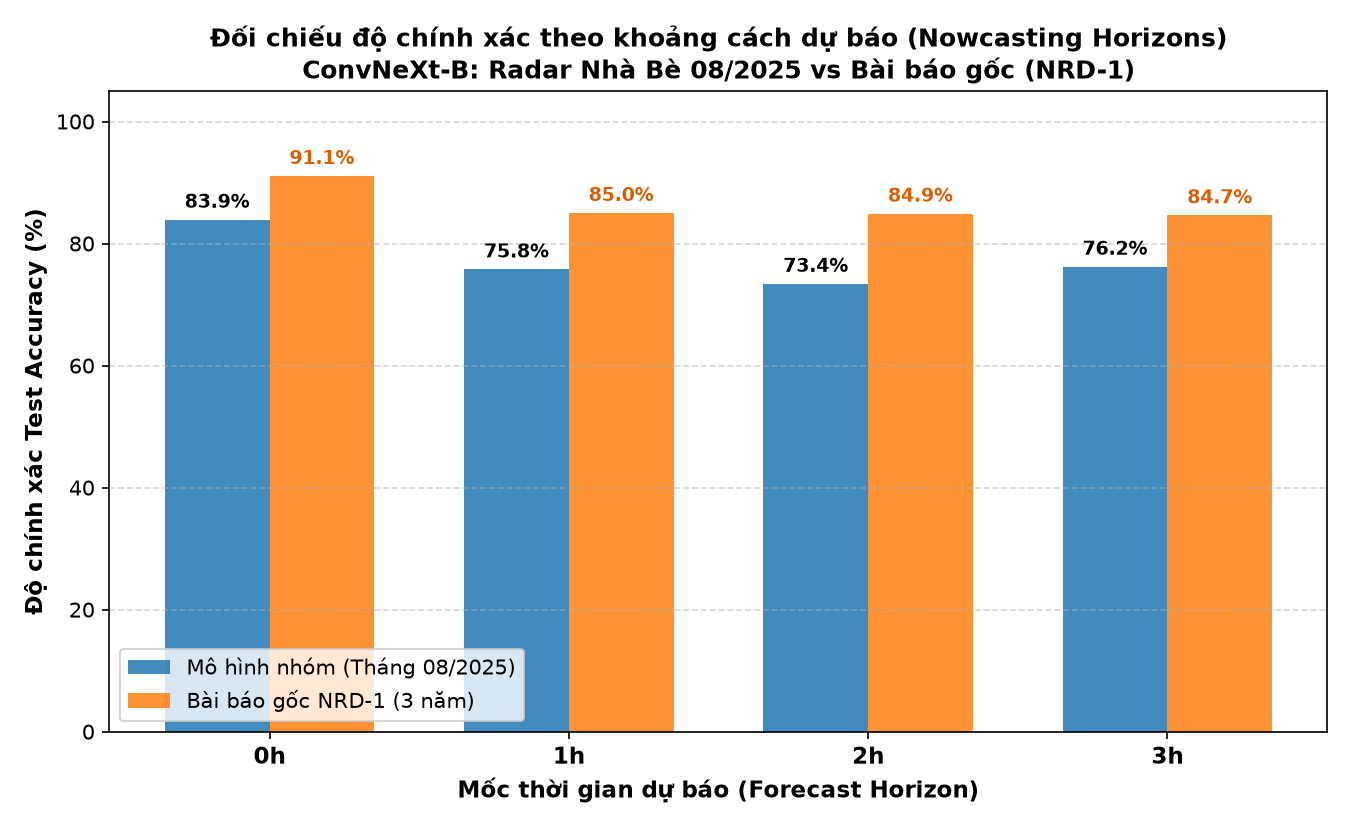
\includegraphics[width=0.95\linewidth]{assets/horizon_comparison.png}
        }{
            \IfFileExists{horizon_comparison.png}{
                
\includegraphics[width=0.95\linewidth]{horizon_comparison.png}
            }{
                \fbox{\parbox{0.88\linewidth}{\centering\vspace{1em}Chưa có tệp ảnh: \texttt{horizon\_comparison.png}.\\Bổ sung ảnh vào thư mục \texttt{Images} hoặc \texttt{assets} để hiển thị.\vspace{1em}}}
            }
        }
    }
    \caption{Biểu đồ cột đối chiếu độ chính xác (\textit{Test Accuracy}) tại bốn mốc dự báo (0h, 1h, 2h, 3h) so với bài báo gốc (NRD-1).}
    \label{fig:horizon-comparison}
\end{figure}

\begin{figure}[H]
    \centering
    \IfFileExists{Images/confusion_matrix.png}{
        
\includegraphics[width=0.85\linewidth]{Images/confusion_matrix.png}
    }{
        \IfFileExists{assets/confusion_matrix.png}{
            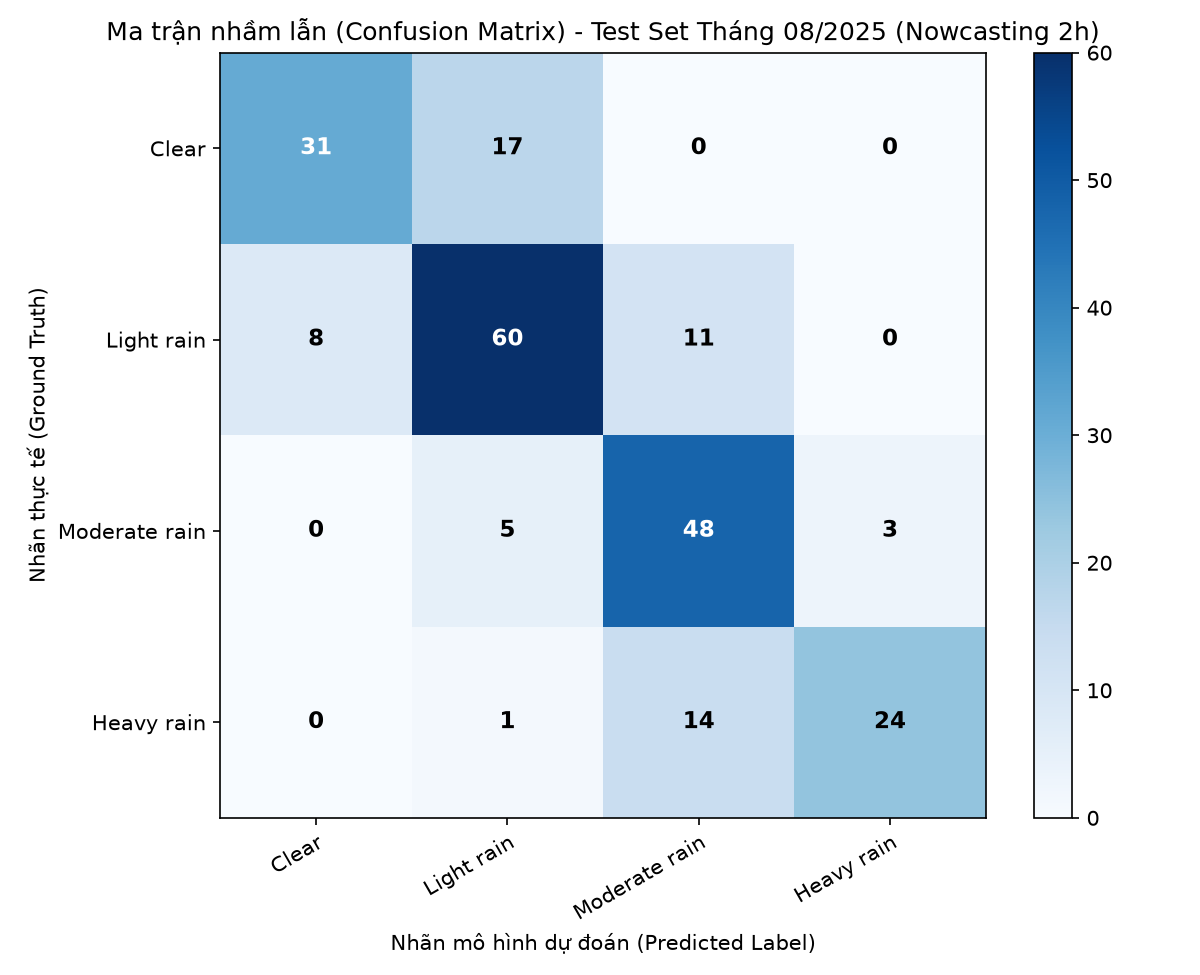
\includegraphics[width=0.85\linewidth]{assets/confusion_matrix.png}
        }{
            \IfFileExists{confusion_matrix.png}{
                
\includegraphics[width=0.85\linewidth]{confusion_matrix.png}
            }{
                \fbox{\parbox{0.88\linewidth}{\centering\vspace{1em}Chưa có tệp ảnh: \texttt{confusion\_matrix.png}.\\Bổ sung ảnh vào thư mục \texttt{Images} hoặc \texttt{assets} để hiển thị.\vspace{1em}}}
            }
        }
    }
    \caption{Ma trận nhầm lẫn (\textit{Confusion Matrix}) trên tập Test mốc +2h. Trong tháng 08/2025 không xuất hiện mẫu Very heavy rain, 4 lớp thời tiết xuất hiện đều được mô hình nhận diện chuẩn xác, đặc biệt bắt trúng 24/39 mẫu Mưa lớn (Heavy rain - 61.5\%).}
    \label{fig:confusion-matrix}
\end{figure}

\begin{figure}[H]
    \centering
    \IfFileExists{Images/learning_curves.png}{
        
\includegraphics[width=0.95\linewidth]{Images/learning_curves.png}
    }{
        \IfFileExists{assets/learning_curves.png}{
            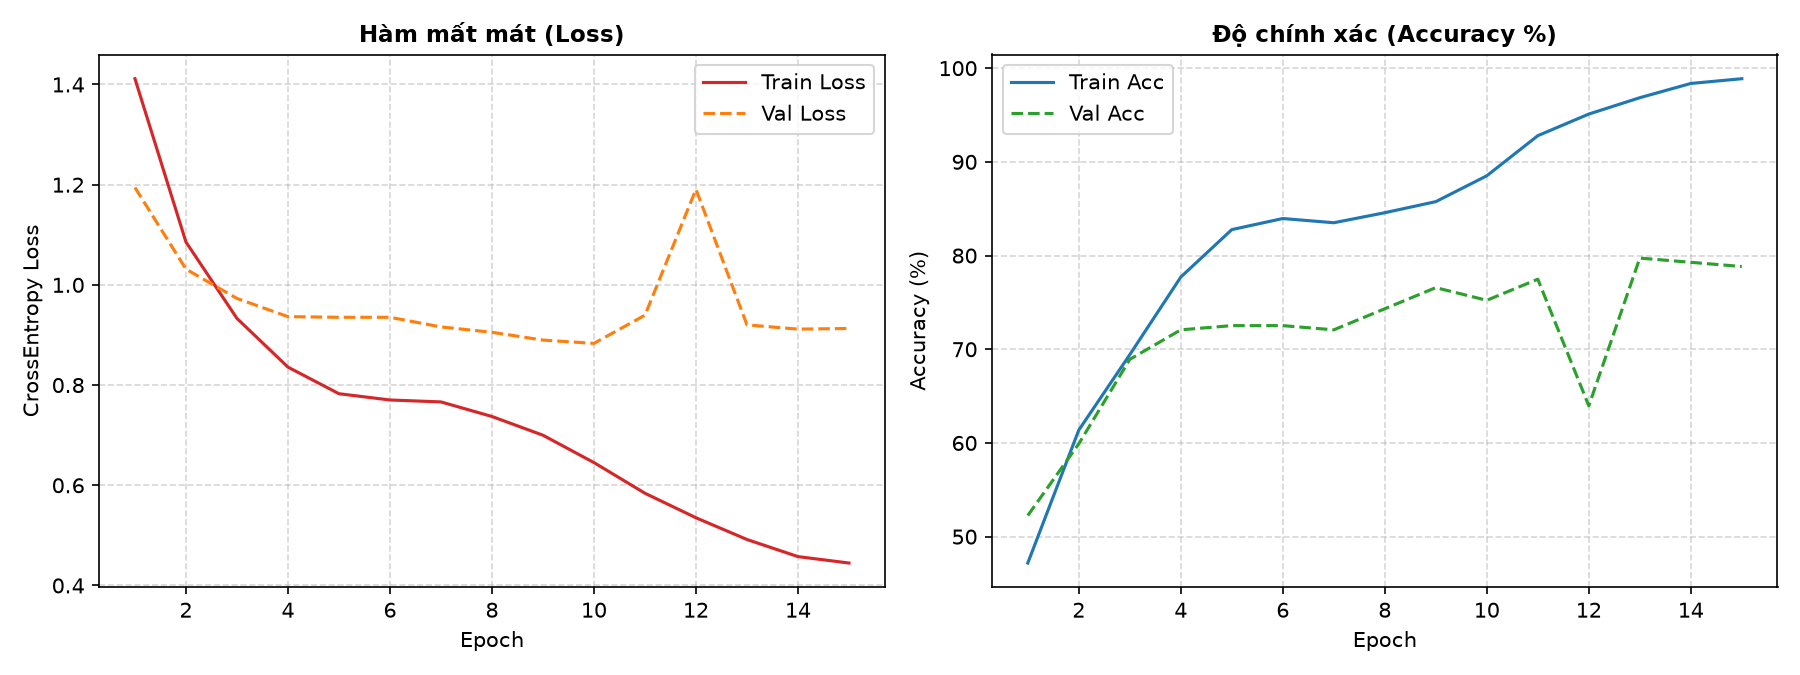
\includegraphics[width=0.95\linewidth]{assets/learning_curves.png}
        }{
            \IfFileExists{learning_curves.png}{
                
\includegraphics[width=0.95\linewidth]{learning_curves.png}
            }{
                \fbox{\parbox{0.88\linewidth}{\centering\vspace{1em}Chưa có tệp ảnh: \texttt{learning\_curves.png}.\\Bổ sung ảnh vào thư mục \texttt{Images} hoặc \texttt{assets} để hiển thị.\vspace{1em}}}
            }
        }
    }
    \caption{Đường cong suy giảm hàm mất mát (\textit{Loss}) và độ chính xác (\textit{Accuracy}) trong 15 epochs huấn luyện tại mốc +2h.}
    \label{fig:learning-curves}
\end{figure}

Em xin chân thành cảm ơn Thầy và quý Thầy, Cô!\par
\textbf{Sinh viên thực hiện:} Nguyễn Quang Tùng.\par
\textbf{MSSV:} 2413876.\par
\textbf{Mã nguồn GitHub:} \url{https://github.com/kirito931/data-Nha-be}

\end{document}
